\chapter{Introduction}
\label{chap:intro}
%%%%%%%%%%%%%%%%%%%%%%%%%%%%%%%%%%%%%%%%%%%%%%%%%%%%%%%%%%%%%%%%%%%%%%%
%%%%%%%%%%%%%%%%%%%%%%%%%%%%%%%%%%%%%%%%%%%%%%%%%%%%%%%%%%%%%%%%%%%%%%%
%%%%%Overview%%%%%%%%%%%%%%
%%%%%%%%%%%%%%%%%%%%%%%%%%%%%%%%%%%%%%%%%%%%%%%%%%%%%%%%%%%%%%%%%%%%%%%
%%%%%%%%%%%%%%%%%%%%%%%%%%%%%%%%%%%%%%%%%%%%%%%%%%%%%%%%%%%%%%%%%%%%%%%

\section{Prelude}
\label{sec: overview}
%what do we have inside galaxies:
% stuff we don't care about because they don't have a big contribution on the SED 1) planets; 2) black holes 3) dark matter
Inside every galaxy, there are millions of stars, planets, and black holes, as well as dust and gas, which all affect each others' formation, evolution and extinction.
There is also dark matter inside every galaxy, which to the best of our knowledge only has gravitational effects on the other components.
Nearly all the information we can obtain from galaxies other than our own comes from their light. % now we can detect gravitational wave which is not part of the SEDs, right? % PB: right.
Young and evolved stars and dust and gas in the space between the stars are the most important contributors to the spectral energy distributions (SEDs) of galaxies. %PB: explain what you mean by spectral energy distribution
We cannot detect any contribution from planets and black holes to SEDs due to their low intensity compared to these other components. %or the limitation of our detectors. % PB: need to rephase a bit  to mention AGN!
Therefore, with properly modeling observed features in SEDs we can extract information about the evolution of stars, dust and gas inside galaxies.

%stars
Arguably, stars are the main component of normal galaxies.
They control the chemical composition and structure of galaxies by transforming gas into new stars and by transforming dead stars back into gas.
They are also central to the formation and evolution of planetary systems.
The energy provided by stars is necessary to create and maintain the life on planets. 
The study of the formation and evolution of the Sun, and more generally that of stars, helps us understand more about our origin and the future of our Solar System.
Furthermore, in order to completely understand the formation and evolution of galaxies from early universe to the current epoch, the knowledge of the formation and evolution of stars is necessary. 
As a result, the study of stellar formation and evolution has been a central topic in astronomy and astrophysics for decades.

%ISM 1)Gas 2)dust
There could be a galaxy without stars (i.e. dark galaxies~\citep[][and references therein]{Cantalupo12}), but there will never be a galaxy without gas. %PB: this is a very strong statement. Some galaxies, like dwarf ellipticals, are pretty gas-free (at least now). So qualify this a bit.
Gas and dust in galaxies can be found in the space between stars that is called the interstellar medium (ISM). The ISM is full of low density gaseous clouds with neutral or ionized atoms and/or molecules, and microscopic dust grains.
The gas and dust in the ISM are heated by interstellar radiation field and cool through a variety of line and continuum processes which usually depend on the local physical conditions. 
The effect of the ISM on stellar formation is undeniable;  it provides the raw material for the formation of stars~\citep[e.g.][]{Kennicutt08,Bigiel08}.
Studying the interstellar medium is not only essential for understanding of the formation of stars, but also it is necessary for interpretation of stellar evolution in that stars release their material into the ISM when they reach the end of their evolution.

% Metallicity %PB: you start talking about metallicity but then switch over to SF. Overview the SF process first, then talk about how metallicity affects it.
Metallicity, which is defined as the ratio of abundance of metals to the abundance of hydrogen, affects formation and evolution of stars indisputably. %PB: define what "metals" means here
In a galaxy like our own, star formation begins with the condensation of giant molecular clouds (GMCs, $\sim 10^7$ M$_{\odot})$ in the ISM due to gravitational instabilities. 
The interplay of turbulence and magnetic fields with self-gravity is believed to be responsible for the formation of clumps within GMCs. 
Some of these clumps develop into self-gravitating cores, which have a similar distribution to stellar initial mass function (IMF) while turbulence and magnetic fields play central roles in defining this distribution (see~\cite{McKee07} for more detail). %PB: this sentence has a lot of concepts in it: going to be hard for non-astronomer to understand
\cite{Walch11} showed that in the case of large scale turbulence, the effect of metallicity on star formation is negligible, but if turbulence is decaying,  metallicity has a strong impact on stabilizing self-gravitating cores. %PB: please check edits to prev sentence
Metals also play an important role in heating, cooling and ionizing processes in the ISM. %%ADD ref.
Since cooling is one of the main reasons for condensation of GMCs~\citep[e.g.][]{Maio07}, in low metallicity regions star formation may be suppressed. %Sahar: should I talk about metallicity in stars and their relation with age? %PB: yes. Need to introduce the general idea of chemical evolution - you hint at this above, but can state it explicitly.

%what does SED look like?
Our primary source of information for galaxies, specifically unresolved ones, is their spectral energy distributions. %PB: since SED is a really important concept, I took out the acronym here.
Broadly speaking, young and hot stars emit most of their light in iltraviolet (UV) wavelengths, evolved stellar populations show themselves in optical and near-infrared (NIR) emission, and gas and dust heated by stellar emission are bright in mid-infrared (MIR) or far-infrared (FIR) wavelengths.
Therefore, UV-to-IR SEDs contain valuable information about galaxies' stellar evolution and their ISM. 
Other wavelengths regimes in galaxy SEDs (i.e. X--ray, radio), that are dominated by processes such as active galactic nuclei, quasars, and supernovae shocks, are beyond the scope of this thesis.
The general shape of SEDs mirrors the morphological type of galaxies; starburst galaxies, which have high star formation rates (SFRs), emit the bulk of their energy in the UV, while the light of quiescent galaxies is dominated by optical and IR emission. 
Detailed information about the age of stellar populations and other properties of galaxies can be determined by modelling their SEDs.

 %how do you model it? %SED model CIGALE %Population synthesis ----> SFR, stellar mass %PB: Need more detail here - how do SED models include SFR, Mstar, etc?
The stellar population synthesis method, which sums stellar spectra of a galaxy to produces its spectrum, has been widely utilized since the 1970s~\citep[e.g.][]{Tinsley72,Searle73} to model SEDs of galaxies.
A through SED model must include stellar population models~\citep[e.g.][]{Bruzual93,Bruzual03,Maraston05}, stellar emission and dust attenuation~\citep[e.g.][]{Calzetti00,Dopita05}, dust grain emission such as from polycyclic aromatic hydrocarbons~\citep[PAHs; e.g.][and references therein]{Tielens08}, and IR emission from gas and dust~\citep[e.g.][]{Chary01,Dale02,Lagache03,Lagache04,Smith07a,Draine07}.%, to fit the observed SEDs.
Many groups have modelled SEDs for different types of galaxies and created SED templates (for more information see the review of \cite{Walcher11} on fitting of SEDs and references therein).
Since the physical parameters of templates generated by the SED models are known, we can find properties of observed galaxies by fitting their SEDs using the templates.
One example of an SED-fitting code is {\em CIGALE}: Code Investigating GALaxy Emission~\citep{Noll09}.
It combines SED models to find the best-fit SED for observed data in the rest-frame UV-to-IR and finds physical properties of galaxies such as SFR, stellar mass and dust attenuation.

%PB: I think you need a one-or-two sentence intro to the overall thesis goals here, so that the reader can see why you are talking about all of this stuff.
In this chapter, we present a review of observational methods of measuring the star formation rate and the main properties that affect measuring and scaling the SFR. A discussion of the ISM and its role in star formation is presented in $\S$~\ref{sec: ism_intro}. In $\S$~\ref{sec: sfr_intro} we discuss measuring the star formation rate, followed by a discussion of the measurement of the stellar mass in $\S$~\ref{sec: starmass_intro}. Current issues about star formation and its relation to other properties of a galaxy are discussed in $\S$~\ref{sec: pre_intro}. 



%%%%%%%%%%%%%%%%%%%%%%%%%%%%%%%%%%%%%%%%%%%%%%%%%%%%%%%%%%%%%%%%%%%%%%%
%%%%%%%%%%%%%%%%%%%%%%%%%%%%%%%%%%%%%%%%%%%%%%%%%%%%%%%%%%%%%%%%%%%%%%%
%%%%%ISM%%%%%%%%%%%%%%
%%%%%%%%%%%%%%%%%%%%%%%%%%%%%%%%%%%%%%%%%%%%%%%%%%%%%%%%%%%%%%%%%%%%%%%
%%%%%%%%%%%%%%%%%%%%%%%%%%%%%%%%%%%%%%%%%%%%%%%%%%%%%%%%%%%%%%%%%%%%%%%


\section{Interstellar Medium} %PB: suggest "Components of the Interstellar Medium in Galaxies" or "The Interstellar Medium in Galaxies"
\label{sec: ism_intro}
%how do we observe it
%what the observation tell us
% how do we measure the dust and gas
The interstellar medium in galaxies is a complex system with a wide range of structures, but these structures can be divided into two main components: gas and dust. %PB: in general, don't start a sentence with an acronym.
The gas in the ISM of galaxies is mostly made of hydrogen and helium with 1 per cent heavier elements (metals), and can be in the form of clouds or diffuse regions.
Gas clouds include molecular clouds, cold neutral atomic hydrogen (\hi) or hot \hi~clouds, and diffuse gas can be either \hii~(ionized hydrogen) regions or hot intercloud medium.
Dust mostly contains silicate, graphite grains can be seen in dark clouds or galactic cirrus.
%Among these regions in ISM, molecular clouds, \hii~regions and dust clouds have important role in understanding star formation in galaxies. 
Emission lines from atoms or ions (i.e \hii~regions) in a hot gas, lines from molecules in cold clouds and 21~cm emission of \hi~are the main observational signatures of the gas in the ISM of galaxies.
Dust can be observed directly through far-infrared and sub-millimeter wavelength emission or indirectly through its extinction and attenuation effects (see Sec.~\ref{sec: extinction}).

Molecular clouds in the ISM are cold ($\sim10$ K) and dense ($ 50<n<500$ cm$^{-3}$); masses of molecular clouds range from a few to millions of solar masses. %~\citep{Bolato08}. %PB: why no citation?
Density in the molecular clouds is not uniform; dense and colds clumps. %PB: I don't get this sentence.
Since these clumps are ideal places to form stars, studying molecular clouds has an important role in understanding formation of stars
However, H$_2$ molecules, the main component of molecular clouds, have no permanent electric dipole moment which makes them difficult to detect in visible light. %PB: just visible light, or all wavelengths?
The second dominant component, helium, is a mono-atomic gas and has the same problem as hydrogen, but these clouds also contain heavier elements such as carbon monoxide, hydrogen cyanide, water, ammonia and more than tens of others.
Carbon monoxide (CO) molecules are the third-most abundant constituent of molecular clouds.
In fact, most of our knowledge from extragalactic molecular clouds comes from observing line emission of CO molecules, which {\bf due to their heavy weight, they have very low rotational state} and can be excited in the temperature of molecular clouds. %PB just extragalactic, or Galactic too? Phrase marked with \bf needs clarification
Other heavier molecules have emission lines which are also detectable in the spectrum of clouds (specially galactic ones), but observing CO emission is the most common way to study the properties of molecular clouds i.e. their mass (see Sec.~\ref{sec: ismmap} for more details).

The molecular clouds are surrounded by clouds of atomic gas~\citep{Kennicutt12}, which are easily traceable by 21-cm emission.
Hydrogen atoms in the ISM (excluding the regions close to hot stars, see below) are in their ground state. 
The electron and proton spins in the ground state can be parallel (i.e. both spin up) or anti-parallel (i.e. the proton's spin is up and the electron's spin is down or vice versa). 
The energy state of the anti-parallel mode is slightly less than the parallel mode.
Since atoms always want to be in the state with lowest energy possible, electrons in the parallel mode have a tendency to flip to the anti-parallel mode. 
However, the difference between these two states is very small and it takes millions of years before the transition happens.
The large amount of hydrogen atoms compensates for the rareness of the transition and at any given time, there are enough hydrogen atoms to emit the 21-cm radiation. 
Observation of the \hi atoms is specifically necessary for understanding physical properties and dynamics of the ISM, which leads to understanding the star formation process~\citep{Walter08}.

\hii~regions are hot and low density regions that are mostly located in the disks of spiral galaxies.
High energy UV photons emitted by massive new born stars have sufficient energy to ionize their surrounding gas, and
~\halpha emission is the main observational feature of \hii~regions.
The temperature and density of these regions can be estimated by observing other recombination lines such as H$\beta$, \sii, \oii, \oiii, and \nii. 
Optically bright \halpha emission from \hii~regions correlates with number of new massive stars in regions and can be used as a star formation tracer~\citep[e.g.][]{Kennicutt98b,Calzetti13}. %PB: moved this sentence.
Studying \hii~regions provides valuable insight into star forming regions by providing information such as star formation rate, initial mass function (IMF), and distribution of ionizing stellar masses~\citep[][and references therein]{Azimlu11}.

%PB: it is difficult to see how the sentences in this paragraph fit together. Right now it reads like a collection of barely-related facts.
Dust has an insignificant effect on the mass of the ISM, but it plays crucial roles in the ISM's evolution.
The total gas mass of galaxies can be determined using optical depth in sub-mm waveband of dust emission. 
In spiral galaxies dust grains are located in cold regions ($\sim 30$~K) and have a power-law distribution of size.
Source of dust thermal emission is from stars and shape of the continuum depends on size of the grain.
Mid-infrared emission from dust grains is mainly dominated by PAHs heated by evolved stellar population~\cite{Smith07a} or recently formed type ``A" and ``B'' stars~\cite{Peeters04}. %PB: A and B or O and B?
Large grains that are either heated by light from star-forming regions or by the interstellar radiation field from total stellar population emit most of their light in far-infrared~\citep[e.g.][]{Calapa14, lu14}
Dust is the main source of extinction and reddening of starlight (See Sec.\ref{sec: extinction} for more information).

\subsection{Map of ISM} %PB: suggest "Mapping the Interstellar Medium"
\label{sec: ismmap}
Measuring the mass of gas in galaxies is a necessary step to know how much raw material is available for forming stars.
A map of the total gas mass in the ISM can be produced by direct observations of gas or using interstellar dust as a tracer. 
Neutral atomic and molecular hydrogen are the most common components of the ISM. %PB: same element
Therefore, to produce a total gas mass map in galaxies, maps of these two components can be added together and multiplied by a constant factor to account for heavier elements which are mostly He. %PB: point out that He can't be observed directly
Another way to do the mapping is to assume that the ratio of total gas to dust is constant across the galaxy, and convert dust observations to a map of total gas mass.

\subsubsection{Direct Measurement of the Gas}

The surface density of gas in the ISM of galaxies can be measured by direct observation of the neutral and molecular hydrogen.
This method can be promising provided that the spatial resolution of observational data is high enough, although due to technical limitations, attaining enough spatial resolution to resolve clouds is almost impossible. This problem shows itself for distant galaxies more than nearby galaxies. 
As a result, using this method is limited and has a lot of uncertainties. % PB last 3 sentences are vague. What exactly ar the limitations and uncertainties? 
 
%\subsubsection{Molecular Clouds}
%PB: some repetition from earlier subsection here. 
The carbon monoxide molecule has a weak permanent electric dipole moment and a ground rotational transition with low excitation energy. 
Given its low energy and critical density, CO can easily be excited even in cold molecular clouds.
Hence CO (usually the $J(1\rightarrow 0)$ rotational transition, observed at 2.6 mm) is used as a tracer of the mass of molecular clouds dominated by molecular hydrogen~\citep[e.g.][] {Sanders84}.
Higher rotational transitions of CO can be used as a tracer as well, but they are not as common as $J(1\rightarrow 0)$.

\cite{Young91} described the relationship between the CO luminosity of a cloud and its mass. The CO luminosity of a cloud is:
\begin{equation}
L_{CO} = D^2 \int I_{\rm CO} d\Omega 
\end{equation}
where $D$ is the distance to the cloud and 
$I_{\rm CO}$ is the CO brightness temperature integrated over the line profile.
It can be written as ${\int T_{\rm CO} dV}$ where $T_{\rm CO}$ is the peak brightness temperature in the CO line and $V$ is the line-width. %PB units for these quantities?
For a uniform cloud with a radius $R$, the CO luminosity is given by:
 \begin{equation}
L_{\rm CO} = \pi R^2 T_{\rm CO} \Delta V
\end{equation}

Galactic molecular clouds are self-gravitating systems. %PB: ref?
Thus, using the virial theorem leads to calculating the mass of the cloud: %(PB note: "Virial" is not a name, no capital needed)
 \begin{equation}
 \label{equ: vir}
 M_{cloud} = L_{\rm CO} \sqrt{\frac{4\rho}{3\pi G T_{\rm CO}}}
 \end{equation}
 where $\sqrt{\frac{4\rho}{3\pi G T_{\rm CO}}}$ is called the conversion factor. %PB: what is \rho here?
 Equation~\ref{equ: vir} shows that the total mass of molecular clouds and the total CO luminosity of a galaxy are directly related~\citep{Young91}. % PB: you refer to individual clouds above, then you jump to totals for the galaxy.  Is this OK to do? (what assumption about optical depth is being made?)
 The relation between CO emission and H$_2$ cloud mass is shown as
%PB: no paragaph break between the text and the beginning of the equation
\begin{equation}
N_{\rm H_2}/\rm cm^{-2} = X_{\rm CO} \times I_{\rm CO}/{\rm K km s}^{-1}
\end{equation}
where X$_{\rm CO}$ is the conversion factor (also known as the X-factor).
The X-factor is different in each galaxy and sometimes is even different in regions within a galaxy due to differences in properties such as metallicity. 
Though assuming a constant conversion factor for galaxies like M82 and M31 can lead to accurate estimation of global molecular gas mass, in regions with low metallicity there are uncertainties. %PB: need references here
Various groups are working on observations of different types of galaxies to measure the X-factor for them~\citep{Wilson95, Bosselli02, Bolato13}.

In order to empirically determine the relation between H$_2$ masses and CO luminosities, many observational attempts have been made on both Galactic and extragalactic scales. 
One of the most significant studies in this regard was done by~\cite{Solomon87}, who studied this relation over more than 273 clouds inside the Milky Way and found a strong correlation between the virial mass of molecular clouds and CO luminosity. 
In Local Group galaxies, several groups have measured size, line width, and CO luminosity of molecular clouds and investigated the relation between  their virial masses and CO emission in environment other than the Milky Way. However, extragalactic investigations were limited to nearby galaxies due to technical problems regarding resolution and sensitivity of the telescopes. 
To measure the clouds in distant galaxies, spatial resolution of maps must be better than 40 pc which is the typical size of a giant molecular cloud~\citep[e.g.][and refrences therein]{Bolato13}. %PB: put these last 2 sentences at end of paragraph
%PB no new paragraph here
Pioneering works in measuring the extragalactic conversion factor were done for M31 and M32~\citep[e.g.,][]{Wilson89, Wilson90}. 
Fig.~\ref{fig: mco} shows the CO luminosity verses virial masses of molecular clouds in the Milky Way, M31, M33, and IC~10. 
The extragalactic molecular clouds are similar to those in the Milky Way. 
The conversion between the CO luminosity and H$_2$ masses is still a controversial topic~\citep[e.g.][]{Narayanan11, Bolato13, Sandstrom13}.
Problems regarding metallicity are not yet solved and it is still not clear whether the conversion factor is global or local. 

\begin{figure}
\label{fig: mco}
\centering
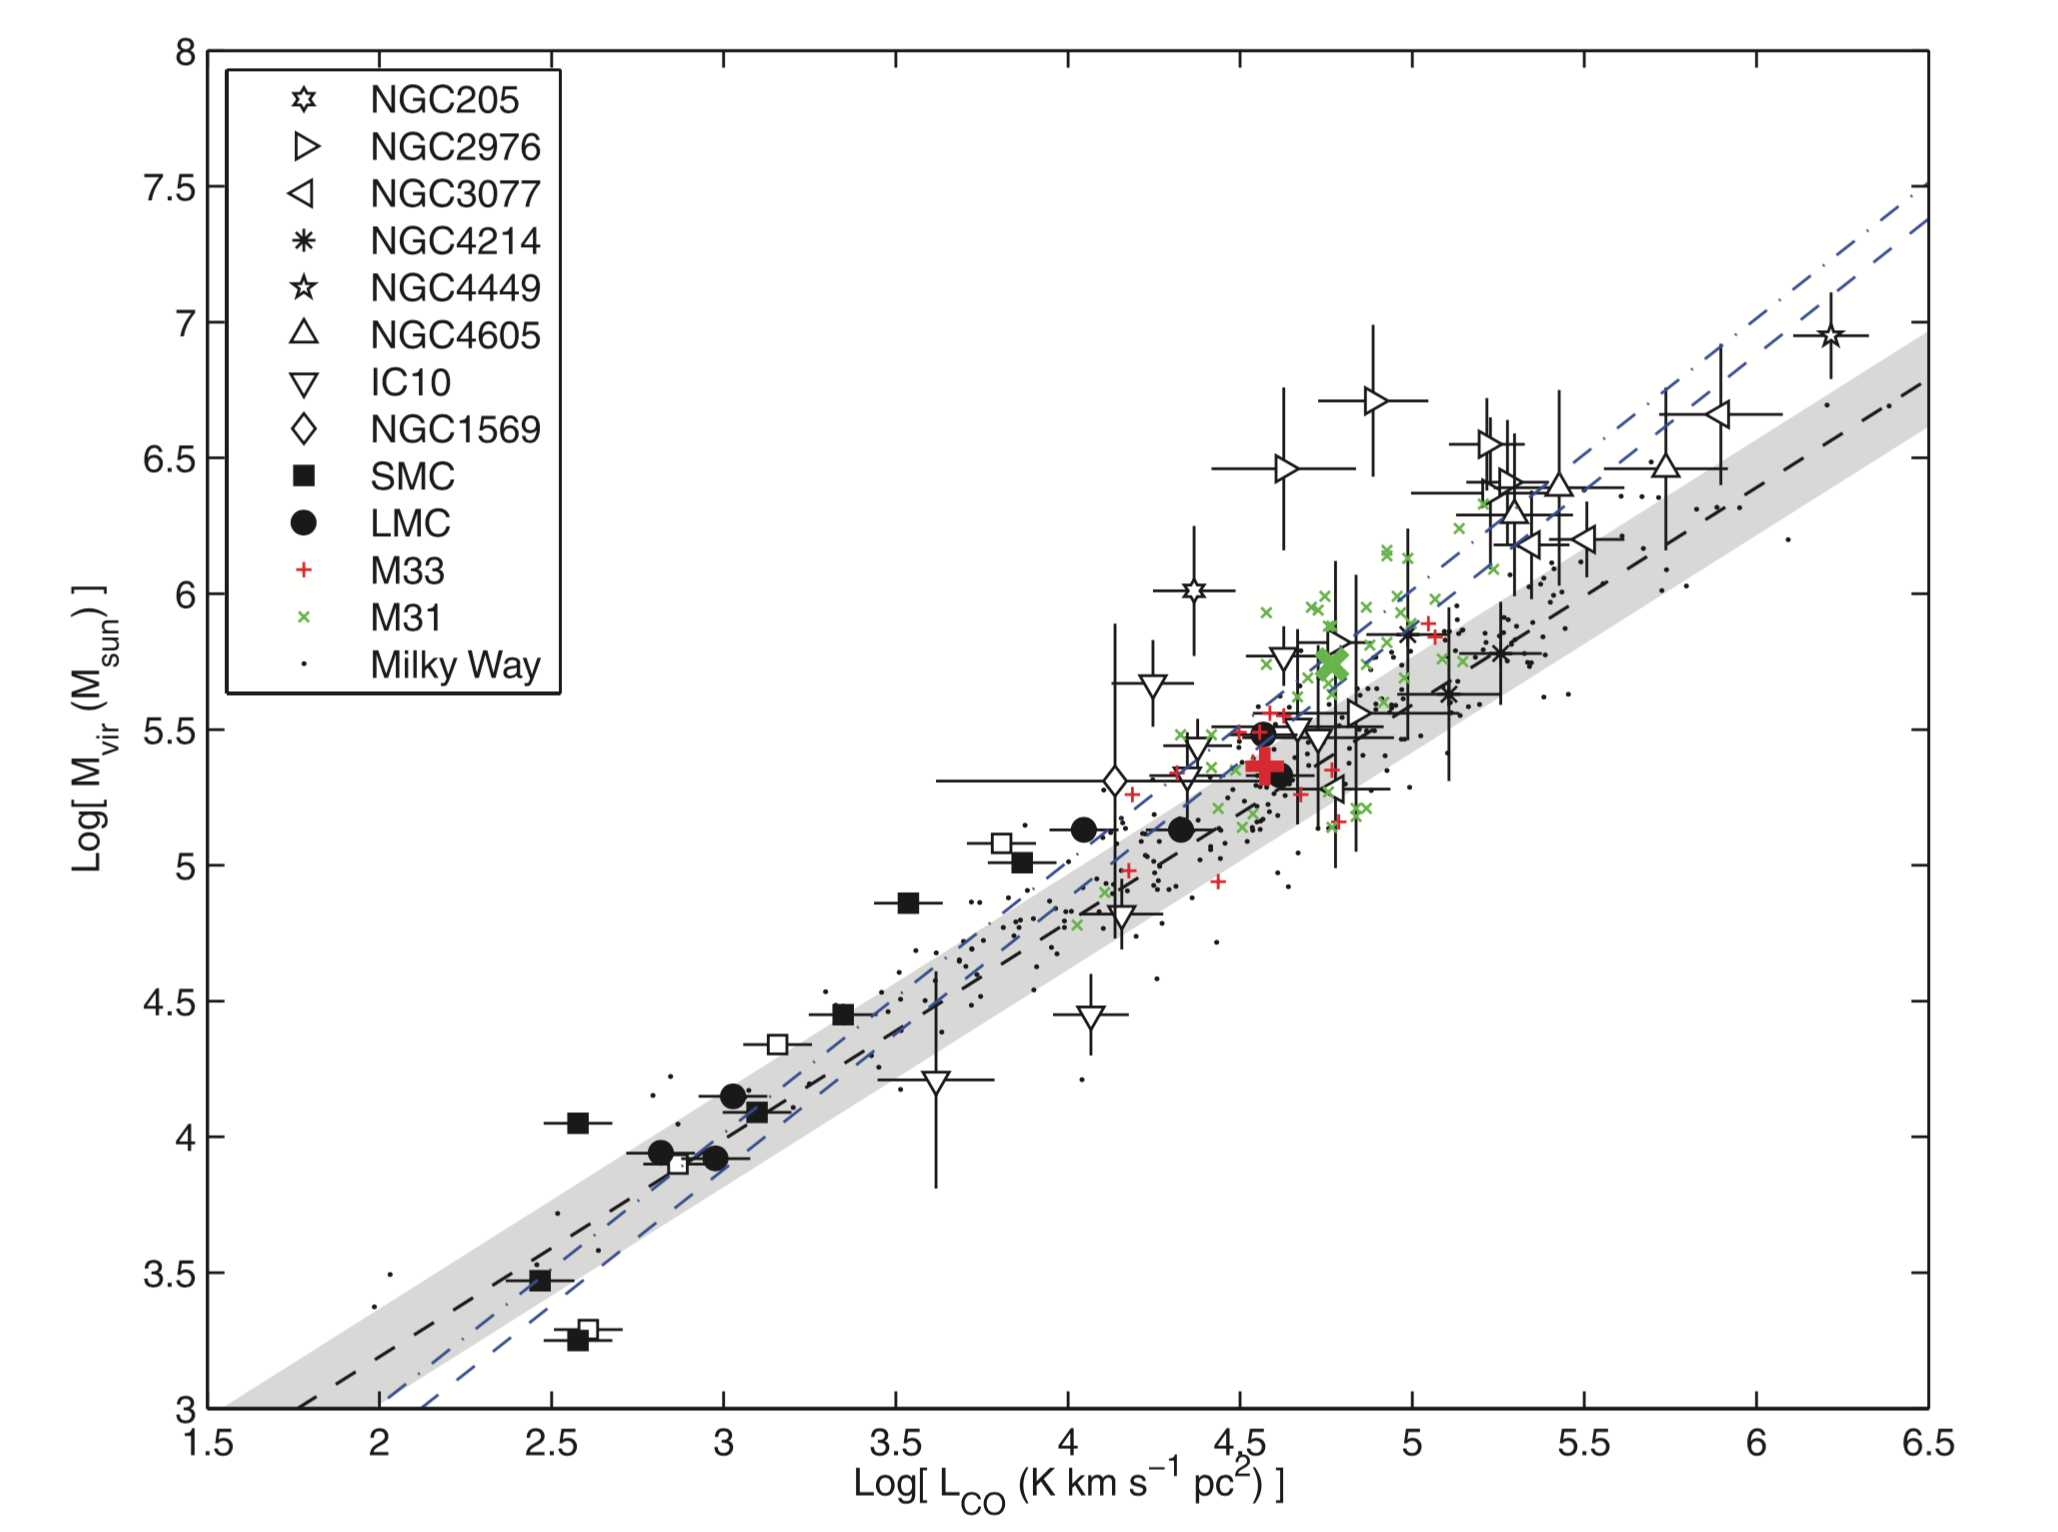
\includegraphics[width=16cm]{../image_intro/mvirial_lco.eps}
\caption{Relation between the virial mass and CO luminosity for the Milky Way (dots), M33 (open circles), M31 (triangles), and IC~10 (squares) clouds. Virial masses are measured from selected high spatial resolution CO observations. The extragalactic molecular clouds are very similar to those in the Milky Way. Adapted from~\cite{Young91}.}
\end{figure}
 
%\subsubsection{Neutral Gas} %PB: paragraph needs a topic sentence
The density of the atomic hydrogen along the line-of-sight is proportional to the intensity of the 21-cm emission. %PB: reverse: intensity of 21cm is proportional to density. Is this optically thin/thick ?
Atomic hydrogen along the line-of-sight contributes to the energy received. %PB does this sentence add something to the previous one?
These properties make the 21-cm line a very useful tool to study gas in the ISM and trace the large-scale distribution of galaxies in the universe (\hi is detectable in most spiral galaxies and some elliptical galaxies).
Although the 21-cm emission is the most reliable technique to map the ISM, the linear relationship between the intensity and the column density of the gas breaks down when the gas is optically thick~\citep{Braun09}. %PB: do you want to give the equation for converting between intensity and mass for HI, the way you did for CO? 

\subsubsection{Dust Emission as a Tracer of Gas} 

Studying the gas clouds in the ISM of distant galaxies by using direct methods is almost impossible and not practical. %PB: why?
\cite{Hildebran83} was the first to suggest that one way to estimate the mass of the gas in the ISM might be from the optical depth of the sub-mm continuum emission from the dust; continuum dust emission is generally optically thin. 
The Herschel Space Telescope \cite{Pilbratt10} measured the continuum dust emission from hundreds of galaxies\citep{Eales10, Oliver12}. 
This amount of observational data provides a unique opportunity to study the ISM of galaxies using dust emission. 
%PB: join these 2 paragraphs
One of the advantages of using the dust emission as a tracer of the gas mass is that unlike the direct method, high spatial resolution is not necessary. %PB: why?
The other important advantage is that this method solves the newly-found problem of the ``dark gas" in galaxies. 
Dark gas is a significant fraction of gas in galaxies which is traced by neither 21-cm emission nor CO emission~\citep{Abdo10}. 
As such it is very difficult to detect with telescopes, but an accurate gas to dust ratio can lead to an accurate estimate of dark gas mass in galaxies. 

There are many disadvantages of the use of the gas to dust ratio to trace gas in the ISM.
In order to use the dust as a tracer of the gas mass, first a relationship between the optical depth and the mass of the dust and then a relationship between the mass of the dust and the mass of the gas must be derived. \cite{Draine03} pointed out that this approach is uncertain because of the uncertainly in the radiative efficiency of dust grains. 
Also, methods of measuring the gas to dust ratio in galaxies are not accurate, which means that there are problems in both steps~\citep{Hildebran83}. 
Using current telescopes, it is difficult to detect dust emission from galaxies at $z > 0.1$~\citep{Ealas12}. %PB: this doesn't seem correct to me - what about submm galaxies?
In some cases such as Virgo cluster galaxies, dust mass is more tightly correlated with the total gas mass than with the masses of molecular or atomic gas separately~\citep{Corbelli11}. %PB: so why is this a problem?

In addition to all the disadvantages mentioned above, the dust method has two major practical problems: firstly, to apply this method, knowing the temperature of the dust is necessary. 
To solve this problem, measurement of the continuum emission at far-infrared wavelengths long enough to cover the peak of the emission must be very accurate~\citep{Ealas12}. 
The other problem is that there is evidence that the gas to dust ratio depends on the metallicity of the gas~\citep{Lisenfeld98, Draine07}, but even in direct methods the dependence on metallicity must be solved. 
%Certainly the gas to dust ratio as a tracer of the total gas in galaxies has a number of problems. PB: sentence doesn't add anything
Unfortunately, at present, given the available devices and technologies, we cannot reach the spatial resolution that is sufficient to detect the gas clouds directly. %PB why do we need high spatial resolution? Or is it sensitivity that is the problem?
Therefore, so far this method is the best available solution for measuring the total gas in distant galaxies. 

\subsection{Extinction and Attenuation} %PB: suggest "The ISM and starlight: extinction and attenuation" or something like that, to make clear why we care about this.
\label{sec: extinction}
In this section, dust ``attenuation" and ``extinction" will be introduced and their effects on measuring the SFR will be briefly discussed. %PB: explain why we care (because stars and dust are spatially mixed in galaxies, and dust affects emitted SED). A  sentence like that is more useful than "in this section we will discuss X".
More advanced and detailed discussion on this topic can be found in the review by~\citep{Calzetti01}. 
Extinction happens when there is a combination of both absorption and scattering of radiation by dust. The distribution of the dust that lies between a source and the observer is irrelevant to the total extinction value because the source is a background point source. %PB: source is *considered* to be a background point source (but what if it isn't a point source?)
% PB: join paragraphs
Attenuation refers to the effects of dust with embedded light sources distributed throughout. 
The dust itself can be clumpy or smooth \citep{Calzetti13}. 
In this situation the relative location of the dust and light sources affect the net absorbed and scattered light, and that happens because both the light sources and the dust have extended distributions. 
Dust scattering's effect depends on whether the dust is in or out of the line of sight. 
When the dust is in the line of sight, attenuation will make the emerging light dimmer and the SED will be bluer. %PB: bluer? really?
This is the typical situation that occurs when studying galaxies or extended regions within galaxies.

To describe the decrease in the intensity of the original beam when it passes through a region where dust particles are present while taking into account the radiation added to the beam by scattering into the line of sight, an integro-differential equation of the radiative transfer of light through dust is used. % PB: "beam" is jargon, change to something else. Simplify this sentence.
At UV/optical/near-IR wavelengths, the radiative transfer equation is: %PB: why does this eqn only apply at UV/opt/NIR? 
\begin{equation}
\frac{dI_{\nu}}{d\tau} = -I_{\nu}  + \frac{a_{\nu}}{\pi} \int I_{\nu}\phi(\nu,\cos \Theta)d\Omega
\end{equation}
where I$_{\nu}$ is the intensity of radiation and $\tau$ is the dust's optical depth.
$a_{\nu}$ is the dust albedo,  the ratio of the scattering coefficient to the sum of the scattering and absorption coefficients. 
$\phi(\nu,\cos \Theta)$ is the scattering phase function, and $\Theta$ is the angle between the scattered photon and the line of sight. %PB: what is \phi? Need to explain at least a little
Both $a_{\nu}$ and $\phi(\nu,\cos \Theta)$ are described in more detail in~\citep{Draine03}. 
The source function, i.e., the dust emission, which usually has small values for wavelengths shorter than a few $\mu$m, is neglected in the equation above. %PB: why no dust emission at short wavelengths? (temperature)
This decrease in the intensity of the stellar radiation must be calculated and corrected for different emission; otherwise, there will be an underestimation of the star formation rate. %PB: what do you mean by "different emission" in this sentence?

%%%%%%%%%%%%%%%%%%%%%%%%%%%%%%%%%%%%%%%%%%%%%%%%%%%%%%%%%%%%%%%%%%%%%%%
%%%%%%%%%%%%%%%%%%%%%%%%%%%%%%%%%%%%%%%%%%%%%%%%%%%%%%%%%%%%%%%%%%%%%%%
%%%%%SFR%%%%%%%%%%%%%%
%%%%%%%%%%%%%%%%%%%%%%%%%%%%%%%%%%%%%%%%%%%%%%%%%%%%%%%%%%%%%%%%%%%%%%%
%%%%%%%%%%%%%%%%%%%%%%%%%%%%%%%%%%%%%%%%%%%%%%%%%%%%%%%%%%%%%%%%%%%%%%%

\section{SFR}
\label{sec: sfr_intro}
Understanding the formation of stars leads to better understanding of galaxies' formation and evolution. 
Characterisation of the star formation processes such as star formation rate (SFR) and the stellar initial mass function (IMF) is necessary in examining galaxies' structure formation~\citep{McKee07}. 
Measuring the SFR is not trivial and depends on a galaxy's morphology, metallicity, IMF, observational spatial resolution, and other properties. 
There is a large number of review papers on how stars form and how their formation is traced. 
From a theoretical perspective, one can refer to the classic picture of the theory of star formation as reviewed by \cite{Shu87} and more recently by~\citep{McKee07}. 
From an observational standpoint, star formation is discussed by \cite[][and references therein]{Kennicutt98b, Kewley02, Calzetti13, Boquien10, Kennicutt12}.

In principle, emission from new stars can be traced by ultraviolet, visible light, near-IR and radio wavelengths, hydrogen recombination lines, forbidden metal lines, and also in the sub-mm range by using the Bremsstrahlung emission. 
Some of this emission is directly from stars, e.g.\ UV emission, and some is from ISM components that absorb and re-emit light from young stars, e.g.\ far-infrared emission.
Techniques to calibrate emission from newly-born stars, preferably hot and massive ones, to the rate at which stars are being formed have been the subject of many studies~\citep[e.g.][]{Calzetti07, Kennicutt11, Hao11,Bigiel08} 
Emission from young, massive, type ``O'' or ``B'' stars is normally used as a tracer of the current SFR. %PB: why?
One of the main assumptions in using the luminosity of massive stars is that the SFR has remained largely constant during the timescale probed by the specific wavelength which is being used as the tracer. 
By knowing the IMF, the number of massive stars can be used to extrapolate the total number of stars formed in a given star-forming region.
To have a reliable SFR indicator, the stellar IMF must be fully sampled to have at least one star in all mass bins (for more detail see Sec.~\ref{sec: imf}).
In general each tracer has some systematic errors, and one should decide which tracer is more accurate for a given system. 

\subsection{Stellar Initial Mass Function}
\label{sec: imf}
One of the most fundamental and difficult questions that a complete theory of star formation must answer is what is the stellar (or cores) initial mass distribution of star forming region. 
Since, most of SFR calibrations use emission from specific mass range stars, it is necessary to know the stellar IMF to determine a more accurate SFR from calibrated photometry data. 
Most problems in modern astrophysical studies regarding the origin and evolution of stars and galaxies can be solved by sampling an IMF ~\citep{Bastin10}. 
\cite{Salpeter55} empirically derived stellar IMF from the observed stellar luminosity function of the Solar neighbourhood~\citep{Shu87}. 
He introduced a power-law IMF in the form of:

\begin{equation}
\label{equ: salp}
\Phi (\log M) = dN / d \log M \propto M^{-\gamma }
\end{equation} 
where M is the stellar mass, $\gamma$ is the power index, and $N$ is the number of stars in logarithmic mass range of $\log M + d\log M$. 

In the late 70s, it was recognised that using the single power-law IMF over all stellar masses is not a correct assumption and might overestimate number of low-mass stars~\citep{Kroupa93, Bastin10}. 
Since then, many groups have studied the stellar IMFs and found different power-law relations for them (Fig.~\ref{fig: imf} ). 
Most SFR calibrations have the same assumption that the stellar IMF is constant across all environments and adopt it from the standard stellar IMF introduced by\cite{Kroupa01}:
\begin{align}
\chi (M) = dN/dM = A M^{-1.3}    \quad    (0.1 \le M(M{\odot}) \le 0.5)\\                  
           = 0.5 A M^{-2.3}    \quad    (0.5 \le M(M{\odot}) \le 100)
\end{align}
where $\chi(M)$ is the number of stars between masses $M$ and $M+dM$. 
Although the Salpeter IMF produces more low-mass stars than the Krupa IMF, they produce almost the same number of the high-mass stars. 
Therefore, the SFR calibrations, which mostly trace massive stars in galaxies, based on the Kroupa IMF and Salpeter IMF can be converted to one another by multiplying the calibration's constant by 1.6~\citep{Calzetti13}. 
In more recent study,~\cite{Weisz15} used data from the Panchromatic Hubble Andromeda Treasury program~\citep[PHAT][]{Dalcanton12} and showed that for nearby galaxies both Kroupa and Salpeter stellar IMF overestimate amount of stars in all masses.
\cite{Bastin10} reviewed the stellar IMF by using many observational results and showed that the stellar IMF is constant and universal, though there are uncertainties in different mass bins especially at the high mass end.


\begin{figure}
\label{fig: imf}
\centering
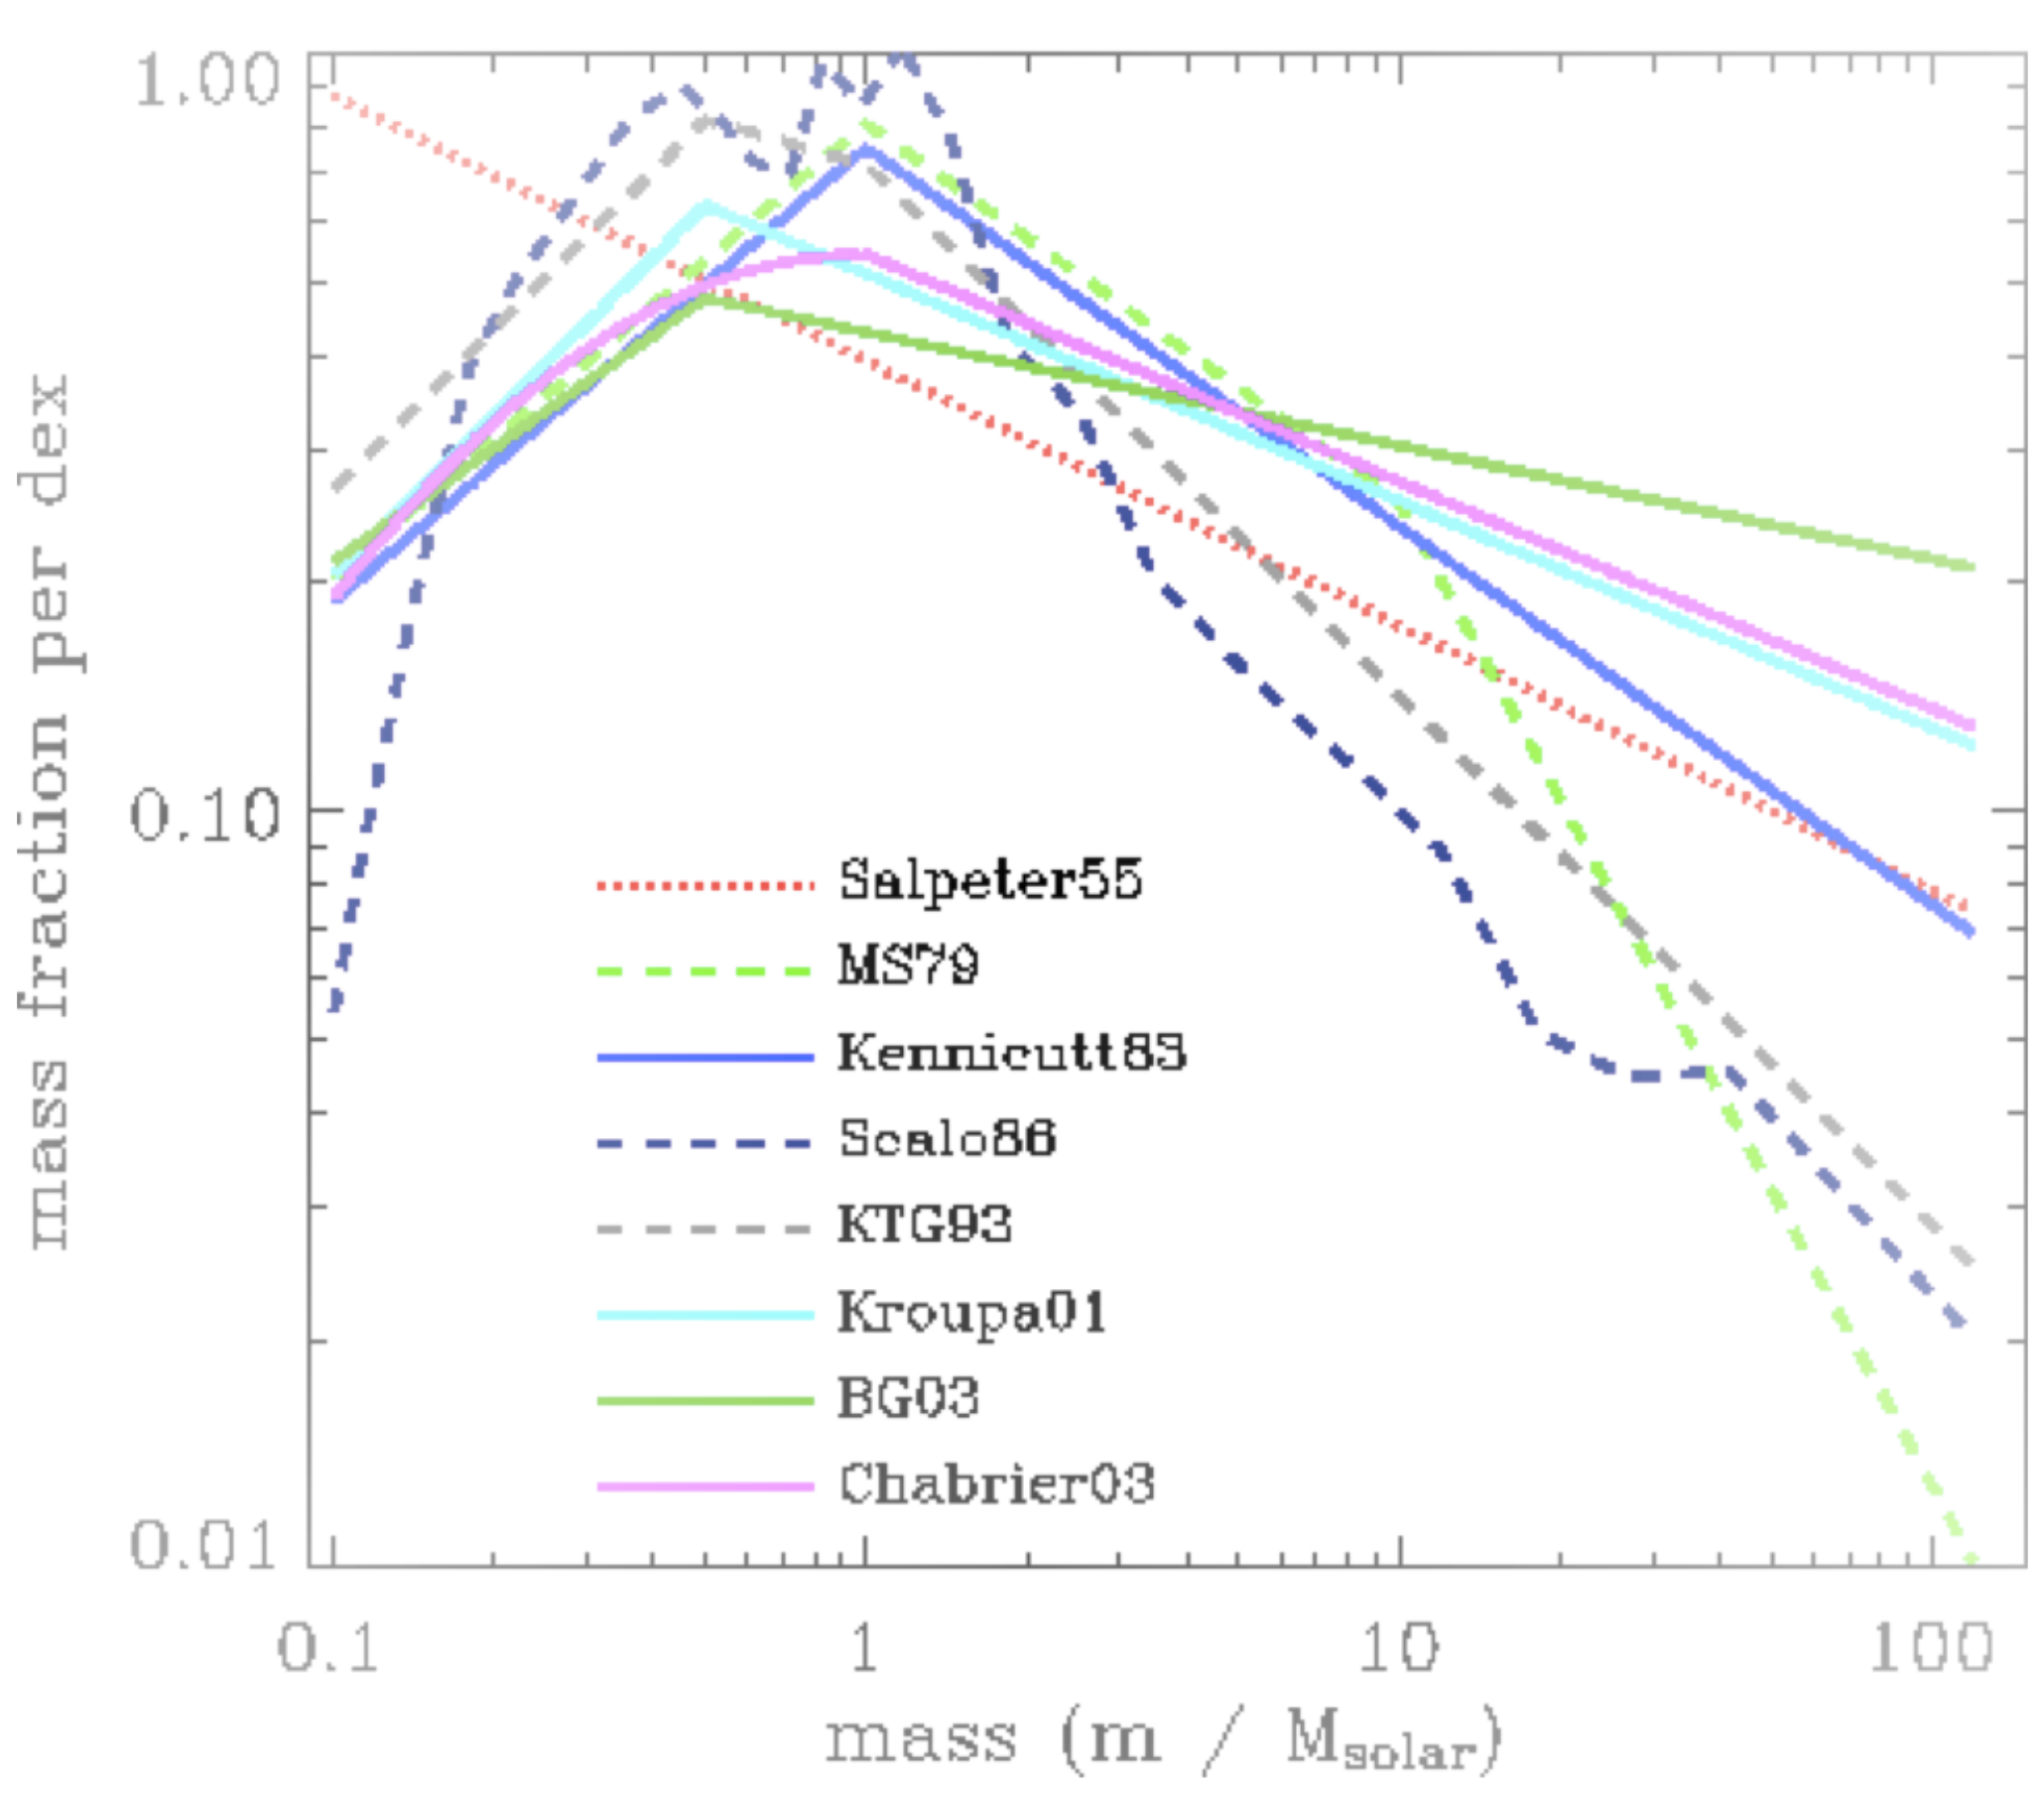
\includegraphics[width=16cm]{../image_intro/imf}
\small
\caption{Comparing the IMFs by plotting the mass fraction per dex versus mass that is normalized so that the integral under each curve is unity. The mass ranges from 0.1 to 120 M$_\odot$. Adopted from~\cite{Baldry03}}
\end{figure}


The careful measurement of the stellar IMF is a key factor in understanding the SFR. 
In distant galaxies, only massive stars can be detected; therefore, the IMF must be measured to include all stellar mass ranges in the SFR calibrations. 
To show the impact of the different stellar IMF assumptions on the SFR calibrations, \cite{Calzetti13} used two different stellar IMFs and derived the SFR calibrations with these new assumptions.
Adopting a modified \cite{Kroupa01} IMF, with its maximum stellar mass set to 30 M$_{\odot}$ instead of 100 M$_{\odot}$, changes SFR calibrations' constants by factors ranging from 1.4 to 5.6 for different SFR indicators (Tab.~\ref{table1}). 

\subsection{SFR Indicators}

One of the main issues to study star formation in distant galaxies is calibration of SFR indicators~\citep[e.g.,][]{Lee10}. 
Calibration of SFR indicators can be affected by differences in star formation history (SFH), metallicity, distribution of stellar population and dust in galaxies~\citep{Calzetti13}. 
Based on the spatial resolution of a system one can divide star formation indicators into two categories: resolved and unresolved star formation indicators.

\subsubsection{Resolved Star Formation Indicators}
The most direct way to measure the SFR and trace recent star formation is counting individual objects~\citep{Kennicutt12}. 
These objects mostly have certain ages and usually are referred to as young stellar objects (YSOs). 
Counting YSOs is a method that used for calculating star formation in molecular clouds within $0.5- 1$ kpc of the Solar System. 
The number of YSOs can be converted to SFR using: 
\begin{equation}
SFR(YSO) = N_{yso} <M>/\tau 
\end{equation}
where N$_{yso}$ is the number of YSOs, $<$M$>$ is the mean mass of YSO which depends on the IMF. 
$\tau$ is the lifetime of the YSO considering some uncertainly $\tau \sim 2$Myr~\citep{Evans09},and the SFR(YSO) is in the unit of M$_{\odot}$yr$^{-1}$. 
Due to observational difficulties, this method can only be applied to the Solar neighbourhood and the Milky Way. 

In theory, for any system with high enough spatial resolution ($\sim 0.5- 1$ kpc), counting YSOs can be used as a tracer of the star formation. 
However, considering the limited capabilities of the present instruments, YSOs in most regions beyond the Magellanic clouds can not be resolved. 
Therefore, most studies use the emission from the energetic ``O" and ``B" stars as a tracer of the SFR. 
Another method to measure the SFR is by looking at the colour-magnitude diagram (CMD) of star-forming regions. 
\cite{Kennicutt12} discusses the new progress made in the spatially-resolved mapping of CMDs to reproduce the spatially and age-resolved maps of star formation in nearby galaxies. 
More detailed studies of CMDs are not in the scope of this paper; for more information, one can refer to~\citep{Kennicutt12}. 

\subsubsection{Unresolved Star Formation Indicators}

 In star-forming regions farther away than the Magellanic clouds, spatial resolution is not high enough to find all the YSOs. 
 In unresolved systems, calibrating continuum or line emission at wavelengths that are sensitive to the young massive stars are primary method of measuring SFR.~\citep[e.g.,][]{Kennicutt98b, Kewley02, Bell03, Calzetti07, Calzetti08, Calzetti10, Calzetti13, Kennicutt07, Kennicutt09, Boquien10, Hao11, Kennicutt12}. 
\cite{Kennicutt98b} calibrated luminosities of galaxies in specific wavelengths for measuring the SFR using relations between the SFR per unit mass or per unit luminosity and the integrated colour of a system provided by synthesis models~\citep[e.g.,][]{Bruzual93}. 

In unresolved systems, the SFR indicators can be divided into local and global ones. 
The global SFR indicators are defined for entire galaxies; therefore, they are luminosity-weighted averages across local star formation history and the physical condition inside each galaxy. 
While local calibration is used for regions within a galaxy, on a scale of sub-galaxy~\citep[e.g.,][]{Zhu08, Kennicutt09, Boquien10, Boquien11, Hao11}.
The limitations in the spatial resolution of the data on the one hand, and the broader applicability of distant galaxy populations on the other, have brought more attention to the calibrations of global SFR compared with the local SFR calibrations that had been done in the past. 
Yet, because of its ability to trace the physical processes of the star formation, local SFR calibration is becoming increasingly important~\citep{Calzetti13}.

\subsubsection*{SFR Indicators Based on the Single-Band Emission}

In order to derive the conversion between the luminosity in specific wavelengths and the SFR, synthesis models are used~\citep{Kennicutt98b}. 
General form of a SFR calibration using single-band emission is: 
\begin{equation}
\label{equ: sfrsingle}
SFR(\lambda)= CL(\lambda)
\end{equation}
where SFR is in units of M${_\odot}$yr$^{-1}$, $L(\lambda)$ is luminosity in erg s$^{-1}$ at the wavelength $\lambda$, and C is the constant derived from stellar population models~\citep[e.g, starburst99][]{Leitherer99}). 
The constant, C, can vary for different emission, mass ranges of the stellar IMF, and the timescale $\tau$ over which star formation needs to remain constant. 
Table~\ref{table1} from \cite{Calzetti13}, summarises the changes in the constant of the calibration. 

\begin{table}
\centering
\caption{Luminosity-to-SFR calibrations adapted from~\cite{Calzetti13}}
\label{table1}
\begin{tabular}{ c c c }
\hline\hline
Luminosity$^1$ & C$^2$ & Assumptions$^3$\\
\hline
L(UV) & $3.0 \times 10^{(-47)} \lambda$ &$0.1 -100 M_{\odot}, \tau \ge 100 Myr $\\
L(UV) & $4.2 \times 10^{(-47)} \lambda$ &$0.1 -30 M_{\odot}, \tau \ge 100 Myr $\\
L(UV) & $4.3 \times 10^{(-47)}\lambda$ &$0.1 -100 M_{\odot}, \tau = 10 Myr $\\
L(UV) & $1.0 \times 10^{(-46)}\lambda$ &$0.1 -100 M_{\odot}, \tau = 100 Myr $\\
L(TIR) & $1.6 \times 10^{(-44)}$ &$0.1 -100 M_{\odot}, \tau = 100 Myr $\\
L(TIR) & $2.8 \times 10^{(-44)}$ &$0.1 -100 M_{\odot}, \tau = 100 Myr $\\
L(TIR) & $4.1 \times 10^{(-44)}$ &$0.1 -30 M_{\odot}, \tau = 100 Myr $\\
L(TIR) & $3.7 \times 10^{(-44)}$ &$0.1 -100 M_{\odot}, \tau = 100 Myr $\\
L(TIR) & $8.3 \times 10^{(-44)}$ &$0.1 -100 M_{\odot}, \tau = 100 Myr $\\
L(H${\alpha}$) & $5.5 \times 10^{(-42)}$&$0.1 -100 M_{\odot},  \tau \ge 6 Myr $\\
L(H${\alpha}$) & $3.1 \times 10^{(-41)}$&$0.1 -30 M_{\odot},  \tau \ge 10 Myr $\\
\hline
\end{tabular}
\begin{tablenotes}
\item $^1$ Luminosities are in erg s$^{-1}$ and are given as $\nu L_{\nu}$.
\item $^2$ The constant C appears in equation~\ref{equ: sfrsingle}. For SFR(UV), the numerical value is multiplied by the wavelength $\lambda$ in $\AA$.
\item $^3$ Assumptions for mass range of the stellar IMF, which we adopt to have the expression derived by \cite{Kroupa01} (see Sec.~\ref{sec: imf}), and for the timescale $\tau$.
\end{tablenotes}
\end{table}


The most common single-band wavelengths that are used as an SFR indicator, is UV emission.
UV emission is an excellent tracer for the SFR due to the fact that the peak of emission for young  ``O" and ``B" stars are in the UV part of the spectrum.
Using spectral energy distribution (SED) from Starburst99, with solar metallicity and assuming~\cite{Kroupa01} stellar IMF with the timescale of over 100 Myr, SFR can be measured as~\citep{Leitherer99}
\begin{equation}
SFR(UV) = 3.0 \times 10^{-47}\lambda L(\lambda)
\end{equation}
where SFR(UV) is in M$_{\odot}$yr$^{-1}$, $\lambda$ in the range of $(912< \lambda < 3000~\AA$), and $L(\lambda)$ is in erg s$^{-1}$. 
As shown in table~\ref{table1}, with changes in the stellar ranges of the IMF, during timescales longer than 100 Myr, the calibration constant only decreases by a few per cent.
However, the calibration constants' changes for shorter timescales are more significant~\citep{Calzetti13}. 
The accuracy of the calibration constant is $\pm 15\%$ which can vary as a function of $\lambda$. 
The UV light can easily be absorbed or scattered by interstellar dust. 
Therefore, using the UV emission as a tracer might lead to underestimating of the SFR, if dust extinction corrections are not applied (\cite{Kennicutt12}; also see Section~\ref{sec: ism_intro}). 

Another single-band SFR indicator is the emission from hydrogen recombination lines. 
Ionizing photons emitted from young massive stars ionize the surrounding gas. Hydrogen recombination line emission, such as the Balmer series lines of H${\alpha}$ $(0.6563 \mu$m) and H${\beta}$ $(0.4861 \mu$m), which are located in the optical wavelength range, are among the most traditional SFR indicators~\citep{Kennicutt98a}. 
The relationship between the intensity of a hydrogen recombination line and the ionizing photon rate for a nebula is derived quantum mechanically. 
To have such results, the nebula must be optically thick to ionizing photons~\citep{Osterbrock06}. 
Being optically thick makes almost all transitions more energetic than Ly${\alpha}$ to be absorbed and re-emited via Ly${\alpha}$ and longer wavelengths.
This is why the H${\alpha}$ emission line strength is greater in optically thick environments. The relation between the SFR, the luminosity of the \halpha emission line and the ionizing photon rate is~\citep[e.g.,][]{Osterbrock06, Kennicutt98b}:

\begin{align}
\label{equ: halpha}
SFR(H\alpha) = 5.5 \times 10^{-42}L(H\alpha) \\
                     = 7.4 \times 10^{-54}Q(H^{\circ})
\end{align}
where SFR(\halpha) is in M$_{\odot}$ yr$^{-1}$, L(\halpha) is in erg s$^{-1}$, and Q(H$^{\circ}$) which is the ionizing photon rate is in units of s$^{-1}$.
The constant at the right-hand side of equation~\ref{equ: halpha} is the resulting coefficient for electron temperature T$_{\mathrm{e}}=10000$~K and density N$_{\mathrm{e}}=100$~cm$^{-3}$ which is the normal case in the interstellar medium. 
All SFR indicators that use the ionization of hydrogen to trace the formation of massive stars are sensitive to the effects of dust.
Dust extinction (Sec.~\ref{sec: ism_intro}) is the most important systematic error for calculating the SFR from hydrogen recombination line.
The effects of dust must be measured and \halpha observations must be corrected or this could lead to underestimating the SFR~\citep{Kennicutt98b}. 

Another nebular line, which is used as a tracer of the SFR is \oii~$\lambda$3727$\AA$.
Although the luminosities of forbidden lines do not correlate with the ionizing atoms directly, their extinction has correlation with the \halpha emission. 
As a result, \oii~luminosity can be used as a tracer of the SFR through \halpha luminosity.
\cite{Gallagher89} calibrated the SFR based on the \oii luminosity by using a sample of 75 galaxies. 
Another calibration for this luminosity was derived by \cite{Kennicutt92}, which has a different calibration factor. 
In his review on the SFR,~\citep{Kennicutt98b} averaged these calibrations and derived the following relation:
\begin{equation}
SFR([O\ II]) = 1.4 \times 10^{-41} L([O\ II])
\end{equation}  
where SFR(\oii) is in M$_{\odot}$ yr$^{-1}$, L(\halpha) is in erg s$^{-1}$. 
Although SFR(\oii) is not as accurate as the SFR(\halpha), it is one of major SFR indicators in high redshift galaxies.
In high redshift galaxies, \halpha emission line is out of optical bands, as a consequence, calibration of the strongest emission feature in the blue light (\oii) as a SFR indicator is really useful~\citep{Kennicutt98b}.


Since interstellar dust absorbs approximately half the starlight and re-emits in the infrared, the IR emission can be used to trace the SFR.
The IR luminosity of a system depends not only on the amount of the embedded dust, but also on the heating rate provided by the stars. 
Since young stars heat the dust to higher mean temperatures than old stellar populations, to the first order the shape of the thermal IR SED depends on the starlight SED~\citep{Helou86}.
The fact that heating rate provided by the young stellar population is higher than the old stellar population indicates that dust heated by the former is more luminous and consequently its SED has peaked at shorter wavelengths (observationally $\approx 60~\mu$m) in comparison with the dust heated by old or low-mass stars.
Therefore, the IR wavelength is able to detect the emission from the young stellar population and be used as an SFR indicator.  

24~$\mu$m and 70~$\mu$m bands are two empirical single-band IR SFR calibrators. 
The use of these two bands depends on the type of the galaxy studied or the physical environment in different regions within the galaxy. 
Since the luminosity of a stellar population with constant star formation increases with time, the IR emission, which is used as a tracer of the emission of the stellar population, has different calibration constants in the case of a global (the entire galaxy SFR indicator) and a local indicator.
That is because the global case includes the Hubble time integrated stellar population of a galaxy, while the other is calculated from regions with short star formation timescales such as: \hii~regions, large star-forming complexes, etc.~\cite{Calzetti13}. 
Table~\ref{table2} shows the constant C from equation~\ref{equ: sfrsingle} for 24~$\mu$m and 70~$\mu$m luminosities and for local (spatial scale $\sim500$~pc for 24~$\mu$m band and spatial resolution less than $\sim 1$ kpc for 70~$\mu$m one) and global cases. 

\begin{table}
\centering
\caption{IR Luminosity to SFR calibrations}
\label{table2}
\begin{tabular}{ c c c c }
\hline\hline
Luminosity$^1$ & C & Assumptions & references\\
\hline
L(24)$^{0.885}_{local}$ & $1.31 \times 10^{(-38)}$ &$(1.10^{40} \le L(24) \le 3.10^{44})$& Calzetti et al. (2007)  \\
L(24)$_{global}$ & $2.04 \times 10^{(-43)}$ &$ (4.10^{42} \le L(24)  \le 5.10^{43})$& Calzetti et al. (2007) \\
L(70)$_{local}$ & $9.4 \times 10^{(-44)} $ &$(5.10^{40} \le  L(70) \le 5.10^{43})$& \cite{Li12} \\
L(70) $_{global}$& $5.9 \times 10^{(-44)}$ &$(L(70) \ge 1.4 \times 10^{42} $& \cite{Li10}\\
\hline
\end{tabular}
\begin{tablenotes}
\item $^1$ Luminosities are in form of L($\lambda$) = $\lambda$ L($\lambda$) in erg s$^{-1}$
\end{tablenotes}
\end{table}  

\subsubsection*{SFR Indicators Based on the Multi-Band Emission}

%%add PAHs here
Despite the usefulness of having single-band SFR tracers, in many cases the corrections due to dust effects and luminosity ranges increases the uncertainty in measurements.
Nowadays, thanks to large surveys, enormous data is available at different wavelengths for galaxies, which allows for combining the emission from different bands and finding new calibrations.
Conversion between SFR and luminosities at different bands mostly helps avoiding problems regarding dust extinction or attenuation (see~\ref{sec: ism_intro}). 
The simplest possible way to combine luminosities at different bands in order to convert them to SFR is through a linear relation, whose correlation with the SFR is empirically proved~\citep{Kennicutt12}. 
%There are studies that use a higher order polynomial relation to combine luminosities~\citep[e.g.,][]{Buat05}; however, this discussion is out of the scope of this paper.

Integrating over the full wavelength range of the IR part of spectrum gives the total infrared (TIR) emission of a system, which can be used as an SFR indicator. 
As mentioned earlier, dust absorbs stellar radiation at all wavelengths; however, here we are only interested in radiation emitted from UV luminous stars. 
It must be noted that since there is no one-to-one mapping between IR and UV emission~\citep{Calzetti13}, it is better to use the TIR emission as a tracer of the SFR instead of single-band IR emission.
 
\cite{Draine07} modelled observations from \Spitzer telescope and found a calibration for TIR luminosity from photometry images instead of using IR SED. 
\cite{Boquien10} tested this calibration and found the modified version of calibration to estimate total infrared luminosity: 
\begin{equation}
L(\rm TIR) = 0.95L(PAH 8 \mu m) + 1.15L(24 \mu m) + L(70 \mu m) + L(160 \mu m)
\end{equation}
where $L = \nu L_{\nu}$ and $L_{\nu}$ is the luminosity  in erg s$^{-1}$ at frequency $\nu$. 
\cite{Calzetti07} indicated that star formation rate calibration for a stellar population undergoing constant star formation over $\tau=100Myr$ is:
\begin{equation}
\label{sfr_tot_IR}
SFR(\rm TIR) = 2.8 \times10^{-44}L(\rm TIR)
\end{equation}
where SFR(TIR) is in M${\odot}$yr$^{-1}$, and L(TIR) is in erg s$^{-1}$. 
To do this calculation, it is assumed that stellar bolometric emission is completely absorbed and re-emitted by dust, i.e., $L_{\mathrm{star}}({\rm bol})=L(\rm TIR)$.

As mentioned before emission from PAHs in ISM can be used as SFR indicator~\citep[e.g.][]{Peeters04}.
Most of studies used MIR emission, which contains PAHs emission, to calibrate SFR~\citep[e.g.][]{Calzetti07}.
\cite{Shipley16} calibrated SFR using observation from 105 star framing galaxies with $z < 0.4$ as:

\begin{equation}
log SFR = A + B log L_{\mathrm{PAH}, \lambda}
\end{equation}
where $L_{\mathrm{PAH}, \lambda}$ is luminosity of PAH features at 6.2, 7.7, 11.3~$\mu$m PAHs features and any combination thereof in erg s$^{-1}$.
Tab.~\ref{table_PAH} shows the constants for each $L_{\mathrm{PAH}, \lambda}$.
These calibration underestimates SFR for low-redshift galaxies with IR luminosity more than $10^12$erg s$^{-1}$.
\cite{Shipley16} showed that adding 7.7~$\mu$m features in calibrations reduces the scatter and concluded that this wavelengths provides the most robust SFR tracer.


\begin{table}
\centering
\caption{SFR calibrations from PAHs luminosities; adopted from~\cite{Shipley16}}
\label{table_PAH}
\begin{tabular}{ l c c}
\hline\hline
PAH Feature(s) & A & B\\
\hline
6.2 + 7.7 + 11.3 & -42.56 $\pm$ 0.03 & 1.00 $\pm$ 0.03 \\ 
6.2 & -40.06 $\pm$ 0.09 & 0.96 $\pm$ 0.04 \\ 
7.7 & -42.38 $\pm$ 0.06 & 1.00 $\pm$ 0.03 \\ 
11.3 & -44.14 $\pm$ 0.08 & 1.06 $\pm$ 0.03 \\ 
6.2 + 7.7 & -42.05 $\pm$ 0.04 & 0.99 $\pm$ 0.03 \\ 
6.2 + 11.3 & -42.52 $\pm$ 0.05 & 1.01 $\pm$ 0.03 \\ 
7.7 + 11.3 & -42.85 $\pm$ 0.04 & 1.01 $\pm$ 0.03 \\ 
\hline
\end{tabular}
\end{table}  

The most common use of combining luminosities to trace the SFR is calibration of the SFR by combination of TIR measurements with both far and near UV observations, with the latter being more commonly used. 
This combination helps to avoid uncertainties from dust attenuation in FUV observations.
\begin{equation}
L_{FUV}(\rm corr) = L_{FUV}(\rm obs) + \alpha L_{\rm TIR}
\end{equation}
where the luminosities are $L = \nu L_{\nu}$ in erg s$^{-1}$, and the coefficient $\alpha$ depends on the bandpasses that are chosen for the UV and IR measurements. $\alpha$ is usually less than 1 because significant amounts of IR emission in many galaxies is from dust heated by older population stars~\citep{Kennicutt12}. The coefficient $\alpha$ is calibrated both theoretically, using evolutionary synthesis models, and empirically, by using measurements of dust corrected SFRs (~\citep[e.p][]{Hao11, Leroy08}. 

Another common method for using the multi-wavelength indicator for star formation is using H${\alpha}$ emission in combination with the 24~$\mu$m emission. 
This combination gives a more accurate dust-corrected estimate of the SFR~\citep{Kennicutt09}:
\begin{equation} 
\label{equ: halphaplus24}
SFR = 7.9 \times 10^{-42}[L(H{\alpha})_{obs} + 0.020L(24)]
\end{equation}
where L(H${\alpha}$)$_{obs}$ is the observed H${\alpha}$ luminosity without correction for internal dust attenuation, given in the unit of erg s$^{-1}$. 
L(24) is the 24~$\mu$m IR luminosity in erg s$^{-1}$, and SFR is in M$_{\odot}$yr$^{-1}$.

\begin{table}
\centering
\caption{Multi-wavelength dust-corrected luminosities, adopted from~\cite{Kennicutt12}}
\label{table3}
\begin{tabular}{ c c}
\hline\hline
Combined luminosities$^1$ & references\\
\hline
L(FUV)$_{corr}$=L(FUV)$_{obs}$ + 0.46L(TIR)& Hao et al. (2011)\\
L(FUV)$_{corr}$=L(FUV)$_{obs}$ + 3.89L(24~$\mu$m)& Hao et al. (2011)\\
L(NUV)$_{corr}$=L(NUV)$_{obs}$ + 0.27L(TIR)& Hao et al. (2011)\\
L(NUV)$_{corr}$=L(NUV)$_{obs}$ + 2.26L(24~$\mu$m)& Hao et al. (2011)\\
L(\halpha)$_{corr}$=L(\halpha)$_{obs}$ + 0.0024L(TIR)& Kennicutt et al. (2009)\\
L(\halpha)$_{corr}$=L(\halpha)$_{obs}$ + 0.020L(24~$\mu$m)& Kennicutt et al. (2009)\\
\hline
\end{tabular}
\begin{tablenotes}
\item $^1$ Luminosities are in form of L($\lambda$) = $\lambda$ L($\lambda$) in erg s$^{-1}$
\end{tablenotes}
\end{table}  
 
Other combinations of luminosities that are used as tracers of the SFR are listed in table~\ref{table3}. 
These composite SFR indicators also have systematic uncertainties; yet, it seems that there is good correlation between multi-band tracers and single-band tracers. 
Moreover, less uncertainty arises in this case than when using the single-band emission as a tracer~\citep{Kennicutt09}. 

As mentioned in section~\ref{sec: imf}, using different IMFs results in having different SFR calibrations' constant. 
From table~\ref{table1} it is clear that changing the IMF affects the H${\alpha}$ SFR calibration more than other SFR calibrations. 
This effect is more than four times larger than UV SFR calibrations because newly-formed stars having up to $\sim 5$ M$_{\odot}$ emit more strongly at UV radiations; however, significant amounts of ionising photons are produced by stars more massive than $\sim 20$ M$_{\odot}$. 
Furthermore, reaching an asymptotic value takes longer for more massive stars (10 Myr for the upper mass limit of 30 M$_{\odot}$ versus 6 Myr for 100 M$_{\odot}$). 
Therefore, changes in the H${\alpha}$ SFR calibration constant are more pronounced, while for UV and TIR calibration constants are fairly close to each other.
On the other hand, using the mean stellar mass for the Kroupa IMF $(<$M$> \sim 0.6$ M$_{\odot})$ yields less than $10\%$ difference between using the upper mass limit of 100 M$_{\odot}$ and 30 M$_{\odot}$. 
As a result, calibrations derived with the mean stellar mass of a system are more accurate than those that are based on tracing the most massive stars~\citep{Calzetti13}.
%%%%%%%%%%%%%%%%%%%%%%%%%%%%%%%%%%%%%%%%%%%%%%%%%%%%%%%%%%%%%%%%%%%%%%%
%%%%%%%%%%%%%%%%%%%%%%%%%%%%%%%%%%%%%%%%%%%%%%%%%%%%%%%%%%%%%%%%%%%%%%%
%%%%%Stellar Mass%%%%%%%%%%%%%%
%%%%%%%%%%%%%%%%%%%%%%%%%%%%%%%%%%%%%%%%%%%%%%%%%%%%%%%%%%%%%%%%%%%%%%%
%%%%%%%%%%%%%%%%%%%%%%%%%%%%%%%%%%%%%%%%%%%%%%%%%%%%%%%%%%%%%%%%%%%%%%%

\section{Stellar mass}
\label{sec: starmass_intro}
One of the most fundamental physical parameters which describes the present state of the galaxies is stellar mass. 
Stellar mass is linked with the structure and star formation history of disc galaxies~\citep{Gavvazi96} and all morphologies~\citep{Scodeggio02}. 
In order to determine stellar population in spiral galaxies, the mean stellar mass density of a galaxy may be a more basic parameter than the total stellar mass~\citep{Bell00}. 
\cite{Kauffmann03} tested that on more than 100,000 galaxies observed by Sloan Digital Sky Survey~\citep[SDSS;][]{York00}. 
They also showed that these results are applied for all morphological types.

Measuring the mass of the stellar population is indirect and subject to significant uncertainties. 
In principle there are two ways to measure stellar mass in galaxies. 
First is measuring the dynamical mass of galaxies using kinematics~\citep{Cappellari06} or lensing~\citep{Auger09}, and then modelling the mass of the dark matter and subtracting it from the measured mass. 
This method has been successful to predict and subtract the mass of the dark matter, which is the dominant mass in galaxies~\citep{Zaritsky94}, and can easily cause uncertainties as high as the order of the measurement. 

The second method is based on stellar population models~\citep[e.g.][]{ Bruzual93, Kotulla09} and using them to connect stellar mass to an observable, like luminosity in different wavelengths, colours, spectral energy distribution from spectroscopy or multi-band observations. 
This method has uncertainties too, and one must also model the uncertainties. 
Uncertainties come from uncertainties in the stellar initial mass function (see Sec.~\ref{sec: imf}), the stellar evolution models, especially the stage where they have most luminosity in their evolution, and the evolutionary state of galaxy~\citep[see,][]{Dalcanton12}, and star formation histories. 

In order to translate between photometry and dynamics the stellar mass to light ratio (M/L) is needed. 
Measuring the accurate M/L can easily lead us to stellar mass surface density.  
To do that, the M/L by can be measured using scale relation between them, from different colours and then multiply it by the surface brightness to calculate the local surface stellar mass density. 
The M/L scale relations make a connection between two methods of measuring stellar mass~\citep{Bell03}. 
These relations are indirect methods for measuring the stellar masses and have high uncertainties in specific cases, but they help to study the stellar mass in large samples. 
This is one of the solution to the problem of the measuring the stellar mass within galaxies. 
As a result it is important to check the accuracy of total stellar mass estimations and provide methods, which measure and produce a map of the stellar mass surface density distribution in galaxies. 
This method gives more accurate result than measuring the stellar mass surface density distribution from single-band images rescaled by uniform mass to light ratio~\citep{Zibetti09}.
 
Having two independent methods to measure stellar mass helps to compare the results and check whether there are any systematic differences. 
Comparing the results from measuring stellar mass in stellar clusters shows there is no huge difference. 
Comparing the results from measuring stellar mass within galaxies shows that the differences are on the order of a few x10 per cent, so one should be more careful to model subtleties~\citep{McLaughlin05}. 

\subsection{Dynamical Mass}
The mass distribution in disk galaxies is usually calculated from rotation curves or integrated line profiles from emission lines such as H${\alpha}$, CO, and \hi lines. 
Thanks to the current generation of detectors, the \halpha and CO lines have very high-resolution spectra over most of the optical disk, and cover most regions in the sky. 
Integrated line widths only yield an estimate of a total mass within some (uncertain) isophotal radius.

Resolved rotation curves produced from \halpha, \hi and CO lines are proportional to optical emission lines within the optical disk of galaxies,~\citep{Courteau13} which helps us to measure the rotational curves. 
The simplest way to estimate the mass of a galaxy is assuming that the physics of the galaxy is the simple Newtonian physics. 
Therefore, the Mass within a potential $\phi$ and the circular velocity in the spherical system is given by:
\begin{equation}
\label{eq: simpmass}
V^2_{circ}(r)=r\frac{d\phi}{dr} = G\frac{M(r)}{r}
\end{equation}
where $M(r)$ is the mass within a sphere of radius $r$. 
For a flattened disk which is the case in most spiral galaxies, the right hand side of equation~\ref{eq: simpmass} must be replaced by the more exact expression derived by~\cite{Freeman70}. 
He assumed in case of no dark matter or bulge, the rotation curve of a self-gravitating disk is:
\begin{equation}
V^2_{circ}(R)= 4\pi G \Sigma_{0}R_{d} y^2[I_0(y)K_0(y) - I_1(y)K_1(y)]
\end{equation}
where $G$ is the gravitational constant, $\Sigma_0$ the central surface brightness, $R_d$ the disk scale length, $4y=\frac{R}{2R_d}$, and $I_i(y)$ and $K_i(y)$ are the first and second kind of modified Bessel functions.

Describing more about calculating dynamical masses in galaxies is beyond the scope of this paper. 
Just note that methods mentioned above is the first order of approximation. 
For more accurate result one should consider that the rotational velocity is not circular and the fact that galaxies contain millions of stars plus interstellar objects therefore simple two object Newtonian physics is not the case here. 
There are lots of different profiles to fit the rotation curve for galaxies.
A detailed review of dynamical mass of galaxies can be found in Courteau et al review paper (2013).

\subsection{Stellar Population Method}
Galaxies can be observed because of their stellar emission and stars radiate the energy produced from nuclear reactions in their cores. 
Given the star's initial mass, the theory of stellar evolution can describe the amount of energy released. 
Hence, stellar mass that is responsible for radiation of stars can be derived by modelling the spectral energy distribution of galaxies. 
However, there is a fraction of mass of evolved stars which no longer emit radiation yet still contribute to the galaxy mass as stellar remnants. 

As mentioned before, stellar population synthesis models is used to reproduce the SED of a stellar population using many physical parameters. 
These parameters, which control the time evolution of the stellar population are:
the age, $t$, of the population, measured in years, also referred to the time passed since the star formation was began;
the star formation history (SFH), often parametrized with SFR $\propto e^{-1/\tau}$; the IM; The metallicity; and the chemical composition ratios, or the fraction of all key elements in galaxies and those values measured in the Sun. 
The stellar evolutionary tracks, the stellar spectral libraries, the parametrization for the mass-loss which affects several late stages of evolution are necessary for stars placing at specific evolutionary phases~\citep{Courteau13}.


%\subsubsection{Calibration light of stars} 
The basic idea behind the finding the suitable calibration between flux/luminosity of the stars in different wavelengths and stellar mass is that one can use the SFHs recovered from synthesizing the stellar optical CMs in different regions in the galaxies. 
The calculated stellar mass can be used to calibrate the fluxes from the stars as the easily measurable parameters of stars. 
Using NIR bands, different groups tried to make a map of stellar mass distributions within galaxies~\citep[e.g.,][]{Elmgreen84}.
Using $B-V$ colours~\citep{Bell01} and $Spitzer$ 3.6- and 4.5-$\mu$m, M/L correction, \cite{Kendall08} produced stellar mass surface densities of M81. 

\cite{Zibetti08} suggested for reaching the maximum spatial resolution one can recombine the photometric information on a pixel-by-pixel study~\citep{Conti03}. 
They used this method to study the stellar mass distribution in galaxies as well as the dependence of the SED on stellar mass density. 
To do so the surface density of stellar mass is derived by 
\begin{equation}
\label{equ: massphot}
\Sigma M_\star (\alpha, \delta) = \Sigma \lambda(\alpha, \delta) \gamma_{\lambda}(\alpha, \delta)
\end{equation}
where $\Sigma \lambda(\alpha, \delta)$ is the surface brightness and $\gamma_{\lambda}(\alpha, \delta)$ is the effective stellar M/L in an effective wavelength $\lambda$. 
In equation~\ref{equ: massphot},  $\gamma_{\lambda}$ can be described as a function of one or more colours as observed at the specified location in galaxy. 
Equation~\ref{equ: massphot} can be used for each position in a galaxy.


\cite{Eskew12} related easily observable quantities to the stellar mass. 
They used 3.6 and 4.5$\mu$m fluxes for calibration of the stellar mass, because these two bandpasses are almost insensitive to the emission from young stellar population, dust absorption and emission. 
Also thanks to \Spitzer~\citep{Wener04} data and WISE~\citep{Wright10} telescopes, great amount of data from many regions in the sky is available, in these bands, which help to test them on more regions and have a more accurate calibration. 
They also test the 3.6- and 4.5 $\mu$m fluxes as proxies for stellar mass in the Large Magellanic Cloud and find the empirical relation between mass of the stars and the luminosities of stars as below:

\begin{equation}
\label{equ:eskew}
M = 31.84 \times 10^{5.65} L_{3.6}^{2.85} L_{4.5}^{-1.85}
\end{equation}
where M$_{\star}$ is the stellar mass and $L = \nu L_{\nu}[\lambda]$ is luminosity in erg s$^{-1}$/$\AA$.
 
\cite{Zhu10} used the SDSS and the $Spitzer$ Wide-area Infrared Extragalactic Survey~\citep[SWIRE;][] {Lonsdale03} to find the calibration between luminosity of the galaxies and stellar masses. 
Using the M/L of galaxies, they found the correlation between $K_s$ band, 3.6 and 4.5 $\mu$m band luminosities and stellar masses and formulate these correlations as:
\begin{align}
\label{equ: zhu1}
\log M_{\star} = (-1.60 ) + (1.12)\times \log \nu L_{\nu}[K_s]\\
\log M_{\star} = (-0.79) + (1.19)\times \log \nu L_{\nu}[3.6\mu \rm m]\\
\label{equ: zhu3}
\log M_{\star} = (-0.25) + (1.15)\times \log \nu L_{\nu}[4.5\mu \rm m] 
\end{align}
where M$_{\star}$ is the stellar mass and $ \nu L_{\nu}[\lambda]$ is the luminosity in erg s$^{-1}$ in specified wavelength. 
Measuring the stellar mass from equation~\ref{equ:eskew} is limited to the nearby galaxies, and might break down for high star forming regions, moreover, this equation have not tested on regions with different metallicity. 
Thus there is no calibration regarding variation in  metallicity~\citep{Eskew12}. 
On the other hand equations~\ref{equ: zhu1} -~\ref{equ: zhu3} have been derived from a large sample of galaxies, and was tested on different type of regions and galaxies. 
Beside they can be used for more distanced galaxy as well as nearby galaxies~\citep{Zhu10}. 
%%%%%%%%%%%%%%%%%%%%%%%%%%%%%%%%%%%%%%%%%%%%%%%%%%%%%%%%%%%%%%%%%%%%%%%
%%%%%%%%%%%%%%%%%%%%%%%%%%%%%%%%%%%%%%%%%%%%%%%%%%%%%%%%%%%%%%%%%%%%%%%
%%%%%Preview%%%%%%%%%%%%%%
%%%%%%%%%%%%%%%%%%%%%%%%%%%%%%%%%%%%%%%%%%%%%%%%%%%%%%%%%%%%%%%%%%%%%%%
%%%%%%%%%%%%%%%%%%%%%%%%%%%%%%%%%%%%%%%%%%%%%%%%%%%%%%%%%%%%%%%%%%%%%%%

\section{Preview}
\label{sec: pre_intro}

Complete picture of galaxies are formed and evolved are tied to unfolding the mystery of formation of stars.
 Various phenomena affect the collapse of molecular clouds and star formation which include environment of the star-forming region, chemical compositions of the region, initial mass distribution of gas, mass of sounding stars and other physical properties of galaxies
 For decades, Observational, theoretical and numerical studies have investigated star formation; nevertheless, their results have never been precise. 
 Empirical studies are used alongside of theoretical ones to find laws that indicate the relations between physical properties of galaxies and star formation.

The most well-known scaling law is the relation between the surface density of FR and the gas surface density, which is known as the Kennicutt-Schmidt (KS) law~\citep{Schmidt59, Kennicutt98a}. 
The K-S law and similar empirical laws were tested on local and high-redshift galaxies with various morphological types, on local and global scales and different ISM types~\citep[e.g][]{Kennicutt08,Bigiel08,Genzel10,Gnedin10,Shi11}.
Despite all these studies, many questions about star formation laws still remain unanswered; the limitations of star formation laws are yet undetermined and there is no definitive answer on whether there is any universal star formation laws.
Their dependence on physical properties of galaxies is nontrivial and sometimes differs by type of star forming regions.
Although relation between stars and gas are well established, the detail of this relation is not clear.
Not only different types of gas change SFR in different ways, but also variations in metallicity for each type alter it.
There is no fully sampled and universal IMF.
In fact there are many debates on weather IMF is universal or not.
Influence of evolved stars and distance of star forming regions from centre of galaxies on SFR is mentioned in studies but not fully investigated.
Besides studying the impact of mentioned properties of galaxies on SFR, searching for other properties of galaxies/star forming regions is continuing.

Advances in observing facilities, image qualities, and methodology expands our knowledge of formation of stars.
Besides these advances, in the past few decades,using advanced statistical methods grew in astronomical studies.
Applying modern statistical methods on star formation studies can shed a light on unsolved problems in this field. 
Studies show that using different statistical methods changes our perspective on star formation laws. 
For example,~\cite{Shetty13} used Bayesian methods to show the K-S law is not universal. 
On the other hand, since astronomy is a data driven science, data mining methods are quiet useful to get new insight on properties of star forming regions.

In this thesis, we present three projects that study effects of quantities of galaxies on SFR.
We use UV to radio observations of both nearby and high-redshift galaxies, measure their physical properties and using modern statistical methods study their impact on SFR.
Chapter~\ref{ch: paper1} focuses on investigating star formation laws in the Andromeda galaxies (M31) in both local and global scales using hierarchical Bayesian analysis.
Additional to the K-S law, we study the extended Schmidt law~\citep{Shi11} and and the metallicity/star formation correlation~\citep{Krumholz09}.
We also show the effect of using different SFR and ISM gas tracers on star formation laws.
In Chapter~\ref{ch: paper3}, we explore nearby galaxies using an unsupervised data mining method (self organizing map, SOM).
We cluster observational data and derived quantities of spatially resolved regions in M31 and examine the physical properties of each cluster.
We find hidden structures in high dimensional data space during this process.
In Chapter~\ref{ch: paper2}, we move to higher redshift and apply SOM algorithm on SED of high-redshift galaxies.
We train networks using a set of galaxy SED templates covering the wavelength range from UV to IR and use them to classify the SEDs of a sample of 142 galaxies with $0.5 < z < 1$. 
Then, we study the grouped properties of classified galaxies.
For each chapter, we also describe the methodology and data used in that chapter.
We summarize our results and discuss potential future work and applications of the results of this thesis in Chapter~\ref{ch: summary}

\addcontentsline{toc}{section}{Bibliography}
\bibliographystyle{apj.bst} 
\bibliography{ref_intro}
